\documentclass[
  bibliography=totoc,     % Literatur im Inhaltsverzeichnis
  captions=tableheading,  % Tabellenüberschriften
  titlepage=firstiscover, % Titelseite ist Deckblatt
]{scrartcl}

% Paket float verbessern
\usepackage{scrhack}

% Warnung, falls nochmal kompiliert werden muss
\usepackage[aux]{rerunfilecheck}

% unverzichtbare Mathe-Befehle
\usepackage{amsmath}
% viele Mathe-Symbole
\usepackage{amssymb}
% Erweiterungen für amsmath
\usepackage{mathtools}

% Fonteinstellungen
\usepackage{fontspec}
% Latin Modern Fonts werden automatisch geladen
% Alternativ:
%\setromanfont{Libertinus Serif}
%\setsansfont{Libertinus Sans}
%\setmonofont{Libertinus Mono}
\recalctypearea % Wenn man andere Schriftarten gesetzt hat,
% sollte man das Seiten-Layout neu berechnen lassen

% deutsche Spracheinstellungen
\usepackage{polyglossia}
\setmainlanguage{german}


\usepackage[
  math-style=ISO,    % ┐
  bold-style=ISO,    % │
  sans-style=italic, % │ ISO-Standard folgen
  nabla=upright,     % │
  partial=upright,   % ┘
  warnings-off={           % ┐
    mathtools-colon,       % │ unnötige Warnungen ausschalten
    mathtools-overbracket, % │
},                       % ┘
]{unicode-math}

% traditionelle Fonts für Mathematik
\setmathfont{Latin Modern Math}
% Alternativ:
%\setmathfont{Libertinus Math}

\setmathfont{XITS Math}[range={scr, bfscr}]
\setmathfont{XITS Math}[range={cal, bfcal}, StylisticSet=1]

% Zahlen und Einheiten
\usepackage[
locale=DE,                   % deutsche Einstellungen
separate-uncertainty=true,   % immer Fehler mit \pm
per-mode=symbol-or-fraction, % / in inline math, fraction in display math
]{siunitx}

% chemische Formeln
\usepackage[
version=4,
math-greek=default, % ┐ mit unicode-math zusammenarbeiten
text-greek=default, % ┘
]{mhchem}

% richtige Anführungszeichen
\usepackage[autostyle]{csquotes}

% schöne Brüche im Text
\usepackage{xfrac}

% Standardplatzierung für Floats einstellen
\usepackage{float}
\floatplacement{figure}{htbp}
\floatplacement{table}{htbp}

% Floats innerhalb einer Section halten
\usepackage[
section, % Floats innerhalb der Section halten
below,   % unterhalb der Section aber auf der selben Seite ist ok
]{placeins}

% Seite drehen für breite Tabellen: landscape Umgebung
\usepackage{pdflscape}

% Captions schöner machen.
\usepackage[
  labelfont=bf,        % Tabelle x: Abbildung y: ist jetzt fett
  font=small,          % Schrift etwas kleiner als Dokument
  width=0.9\textwidth, % maximale Breite einer Caption schmaler
]{caption}
% subfigure, subtable, subref
\usepackage{subcaption}

% Grafiken können eingebunden werden
\usepackage{graphicx}
% größere Variation von Dateinamen möglich
\usepackage{grffile}

% schöne Tabellen
\usepackage{booktabs}

% Verbesserungen am Schriftbild
\usepackage{microtype}

% Literaturverzeichnis
\usepackage[style=alphabetic,]{biblatex}
% Quellendatenbank
\addbibresource{lit.bib}

% Hyperlinks im Dokument
\usepackage[
  unicode,        % Unicode in PDF-Attributen erlauben
  pdfusetitle,    % Titel, Autoren und Datum als PDF-Attribute
  pdfcreator={},  % ┐ PDF-Attribute säubern
  pdfproducer={}, % ┘
]{hyperref}
% erweiterte Bookmarks im PDF
\usepackage{bookmark}

% Trennung von Wörtern mit Strichen
\usepackage[shortcuts]{extdash}

\title{V504: Thermische Elektronenemission}
\author{
  Simon Schulte
  \texorpdfstring{
    \\
    \href{mailto:simon.schulte@udo.edu}{simon.schulte@udo.edu}
  }{}
  \texorpdfstring{\and}{, }
  Tim Sedlaczek
  \texorpdfstring{
    \\
    \href{mailto:tim.sedlaczek@udo.edu}{tim.sedlaczek@udo.edu}
  }{}
}
\publishers{TU Dortmund – Fakultät Physik}

\date{Durchführung: 23.05.2017\\
      Abgabe: 30.05.2017}


\begin{document}

\maketitle
\thispagestyle{empty}
\tableofcontents
\newpage
\setcounter{page}{1}
\section{Zielsetzung}
\label{sec:zielsetzung}
Ziel des Versuchs ist es, durch Erwärmung einer Metallfläche, freie Elektronen aus dieser zu emittieren.
\section{Theorie}
\label{sec:theorie}
Die Elektronenemmision aus einer Metallfläche wird auch als glühelektrischer Effekt bezeichnet. Die Grundlage, um diesen Effekt zu beobachten ist die Austrittsarbeit der Metalloberfläche zu überwinden. Die innere Energie der Elektronen muss somit etwa gleich groß wie die Austrittsarbeit sein, damit diese die Metalloberfläche verlassen können. Dieser Effekt ist temperaturabhängig. Daher werden in diesem Versuch fünf Kennlinien mit fünf verschiedenen Heizströmen und Heizzspannungen aufgenommen.
\begin{figure}[htb]
  \centering
  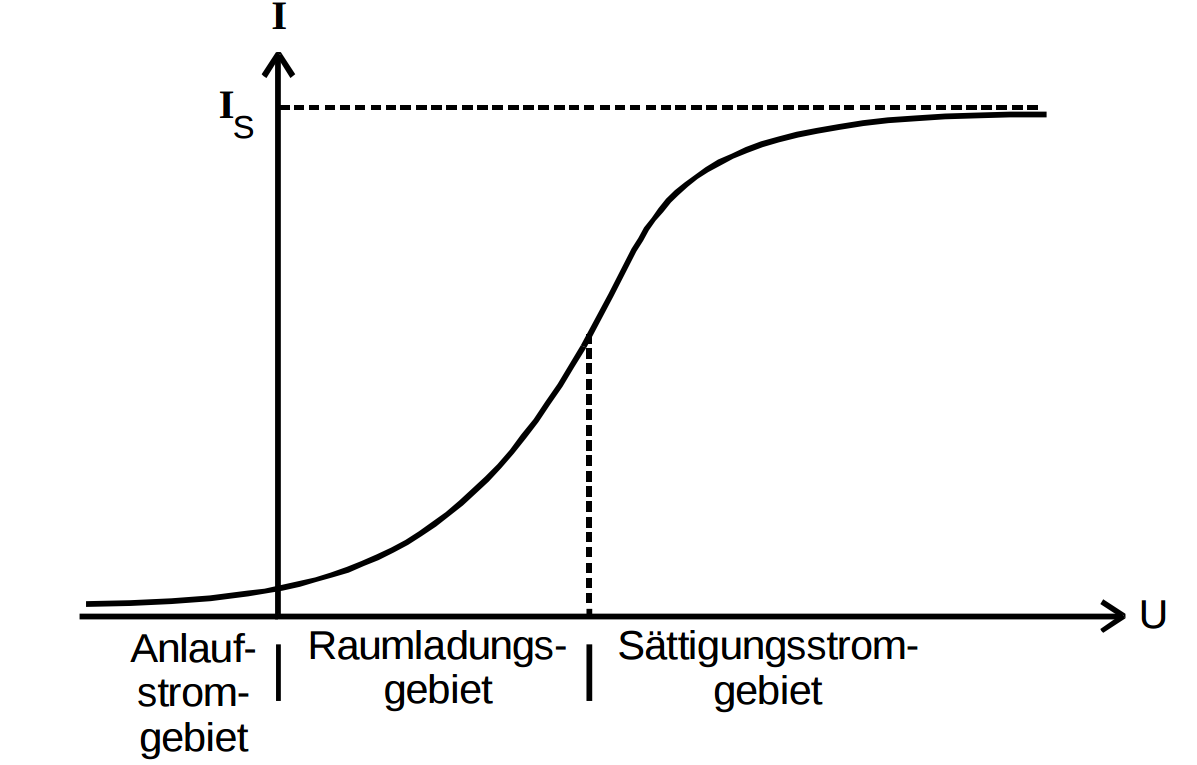
\includegraphics[width=0.9\textwidth]{V5044.png}
  \caption{Der Graph einer Kennlinie. \cite{anleitung}}
  \label{fig:V5044}
\end{figure}
\noindent
Abbildung \ref{fig:V5044} zeigt eine übliche Kennlinie. Dabei wird prinzipiell  die Spannung zwischen Anode und Kathode gegen den fließenden Strom abgebildet. Logischerweise muss das Experiment in einem Vakuum durchgeführt werden, da sonst Teilchen miteinander wechselwirken könnten und somit die Messungen verfälschen würden. Abbildung \ref{fig:V5045} zeigt den Aufbau einer in diesem Versuch verwendeten Diode.
\begin{figure}[H]
  \centering
  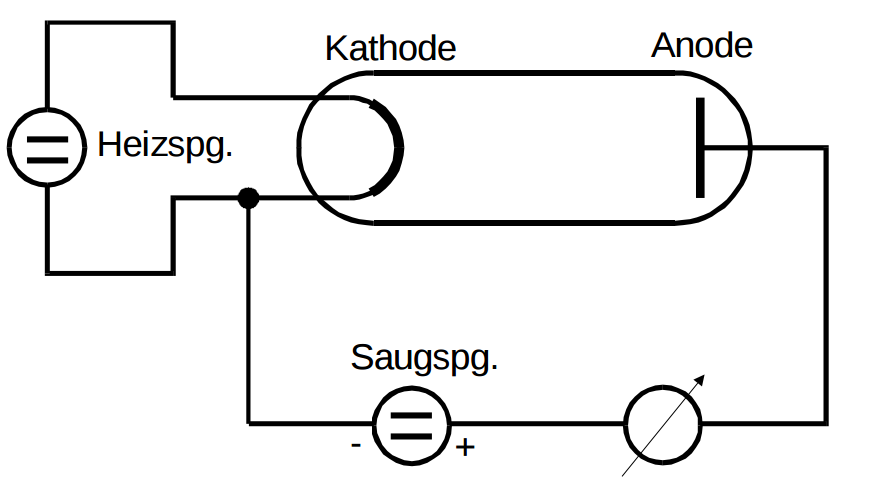
\includegraphics[width=0.9\textwidth]{V5045.png}
  \caption{Der Versuchsaufbau einer Hochvakuumdiode. \cite{anleitung}}
  \label{fig:V5045}
\end{figure}
\noindent
Zu sehen ist, dass der Graph in Abbildung \ref{fig:V5044} drei Teilgebiete aufgeteilt ist. Zum ersten das Anlaufstromgebiet, indem selbst für kleine Gegenspannungen noch ein Anodenstom vorgewiesen werden kann. Dieser Effekt ist darauf zurückzuführen, dass die Elektronen eine Eigengeschwindigkeit beim Verlassen der Kathode besitzen. Dabei ergibt sich für die Stromdichte der Gegenspannung $V$ der Zusammenhang
\begin{equation}
  j(V)\,=\,const\,\exp\Big(-\frac{e_0V}{kT}\Big).
  \label{eqn:stromdichte}
\end{equation}
Nach dem Anlaufstromgebiet folgt das Raumladungsgebiet. Nach der Gleichung
\begin{equation}
  j_S (T)\,=\,4\pi \frac{e_0 m_0 k²}{h³} T² exp\Big(-\frac{e_0 \phi}{kT}\Big)
  \label{eqn:richardson}
\end{equation}
ist die Zahl der pro Zeiteinheit emittierten Elektronen nicht von der Anodenspannung abhängig, sondern lediglich von der Temperatur. Dadurch ist das Raumladungsgebiet nicht für beliebig hohe Anodenspannungen gültig. Die Stromdichte $j$ ist an jeder Stelle konstant, aber gegeben durch
\begin{equation}
  j\,=\,-\rho v.
  \label{eqn:j}
\end{equation}
Daraus folgt, dass die Raumladungsdichte $\rho$ den Verlauf der Feldstärke zwischen Anode und Kathode beeinflusst. Daher gilt das Langmuir-Schottkysche Raumladungsgesetz:
\begin{equation}
  j\,=\,\frac{4}{9} \epsilon_0 \sqrt{\frac{2e_0}{m_0}}\,\frac{V^{\frac{3}{2}}}{a^2}.
  \label{eqn:raumladung}
\end{equation}
\noindent
Durch eine wachsende Gegenspannung wird der Anodenstrom einem Sättigungswert zustreben. Das darauffolgende Gebiet nennt sich dann Sättigungsstromgebiet. In diesem Bereich erreichen alle Elektronen die Anode.
\section{Durchführung}
\label{sec:durchführung}
\subsection{Versuchsaufbau}
\label{sec:aufbau}
Abbildung \ref{fig:V5041} zeigt den Versuchsaufbau zur Aufnahme der Kennlinien.
Die Kathode der Diode wird dafür durch den Heizstrom erwärmt. Dadurch emittiert diese dann Elektronen, die mit Hilfe der Anodenspannung $U_A$ dann zur Anode gelangen.
\begin{figure}[H]
  \centering
  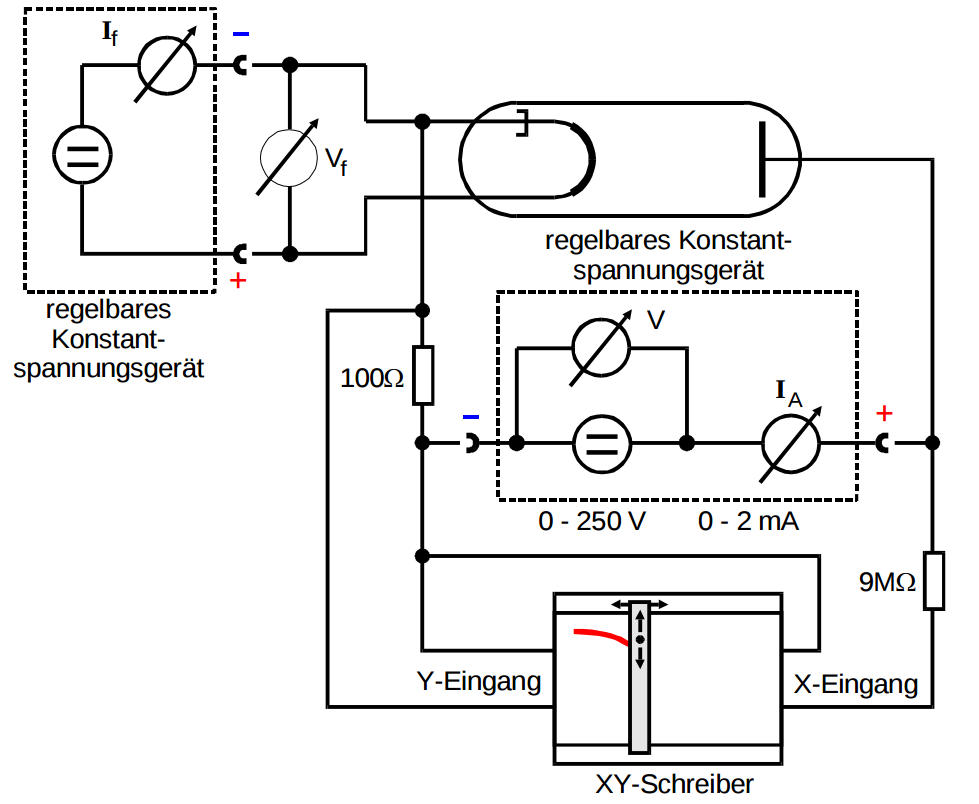
\includegraphics[width=0.9\textwidth]{V5041.png}
  \caption{Der Versuchsaufbau zur Aufnahme der Kennlinien. \cite{anleitung}}
  \label{fig:V5041}
\end{figure}
\noindent
Es wird ein Konstantspannungsgerät benutzt, welches den Heizstrom $I_f$ liefert, der am eingebauten Amperemeter abgelesen werden kann. Dieses ist mit der Diode verbunden, welche die Kennlinien liefert. Es ist außerdem ein weiteres regelbares Konstantspannungsgerät im Schaltkreis verbaut. Mit diesem wird die Anodenspannung $U_A$ bestimmt. Einen XY-Schreiber gab es allerdings nicht.\\
\\
In Abbildung \ref{fig:V5042} ist der Versuchsaufbau zur Aufnahme der Anlaufstromkurve zu sehen.
\begin{figure}[H]
  \centering
  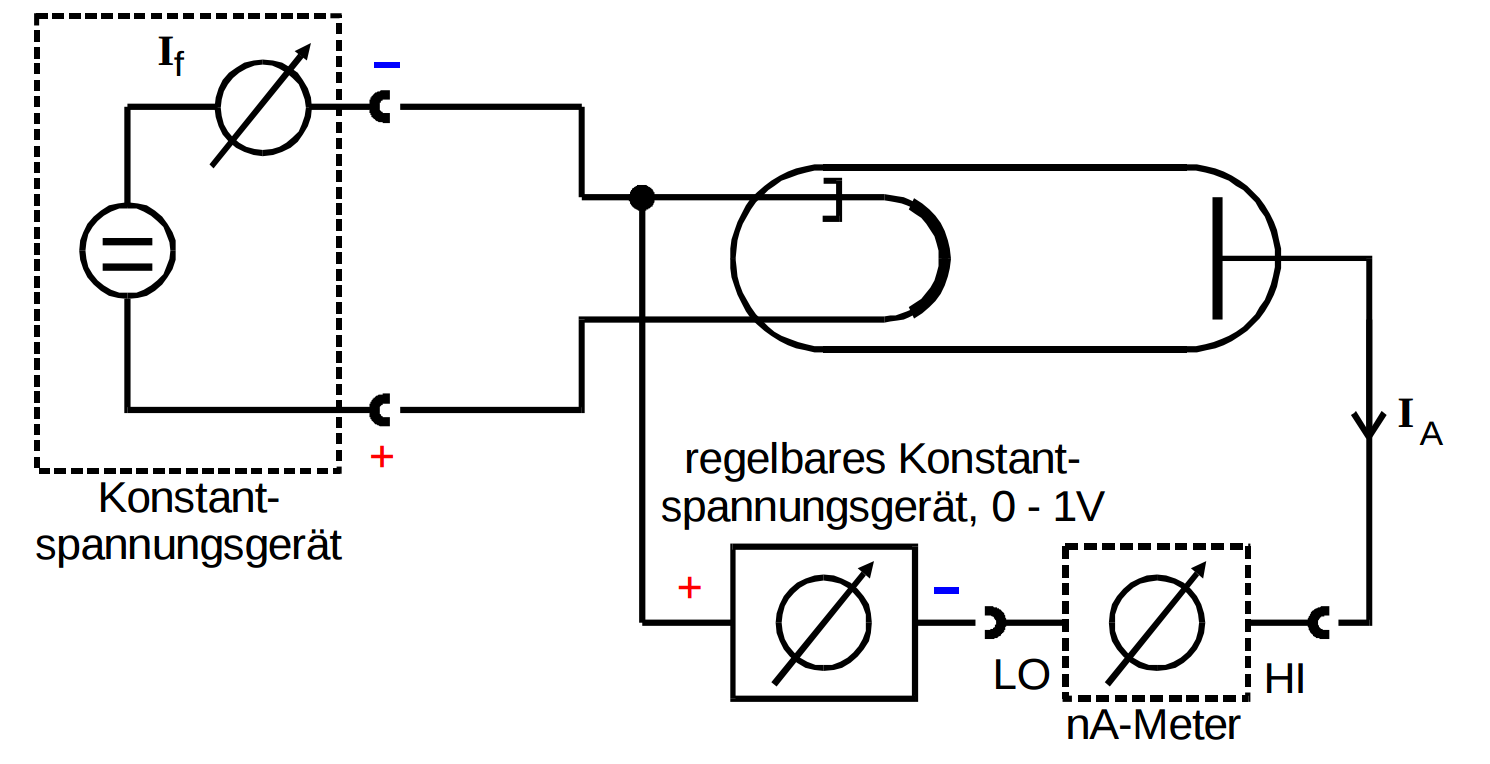
\includegraphics[width=0.9\textwidth]{V5042.png}
  \caption{Der Versuchsaufbau zur Aufnahme der Anlaufstromkurve. \cite{anleitung}}
  \label{fig:V5042}
\end{figure}
\noindent
Auch hier ist wieder ein Konstantspannungsgerät verbaut, welches für einen konstanten Heizstrom $I_f$ sorgt. Außerdem ist dieses erneut mit der Diode verbunden, welche allerdings nun mit einem Konstantspannunggerät verbunden ist, welches lediglich Spannungen zwischen \SI{0.1}{\volt} und \SI{0.96}{\volt} erzeugen kann. Außerdem ist die Diode mit einem Nanoampere-Meter verschaltet.
\subsection{Versuchsablauf}
\label{sec:ablauf}
Zuerst werden die Geräte, wie in Abbildung \ref{fig:V5041} dargestellt, verschaltet. Danach werden 5 mal 40 Werte für die Anodenspannung $U_A$ und für den Anodenstrom $I_A$ gemessen. $U_A$ befindet sich währendessen stets zwischen \SI{0}{\volt} und \SI{250}{\volt}. Die Heizspannung $U_f$ und der Heizstrom $I_f$ werden vor jedem Durchgang von 40 Messungen jeweils bestimmt und bleiben konstant. Danach werden 10 Werte für $I_A$ aufgenommen, um daraus unter anderem die Anlaufstromkurve zu bekommen. Dabei befindet sich $U_A$ währendessen stets zwischen \SI{0.1}{\volt} und \SI{0.96}{\volt}. Das Messgerät hat dabei einen Innenwiderstand von \SI{1}{\mega\ohm}.
\end{document}
